% Perturbation Diagram TikZ Macros

% Some style definitions
\tikzstyle{block} = [rectangle, draw, text centered]
\tikzstyle{line} = [draw, -latex]
\tikzstyle{vec} = [draw, -latex, dashed]
\tikzstyle{mmat} = [draw, -latex, double]
\tikzstyle{mvec} = [draw, -latex, double, dashed]
\tikzstyle{tensor} = [draw, -latex, dashdotted]

% First argument is name, second is location specifier
\newcommand{\addb}[2] { \node[block, #2] (#1) {$+$}; }
\newcommand{\mulb}[2] { \node[block, #2] (#1) {$*$}; }
\newcommand{\invb}[2] { \node[block, #2] (#1) {$-1$}; }
\newcommand{\eigb}[2] { \node[block, #2] (#1) {$\lambda$}; }
\newcommand{\evecb}[2] { \node[block, #2] (#1) {$\xi$}; }
\newcommand{\svecb}[2] { \node[block, #2] (#1) {$\nu$}; }
\newcommand{\rotb}[2] { \node[block, #2] (#1) {$\circlearrowright$}; }
\newcommand{\whiteb}[2] { \node[block, #2] (#1) {$W$}; }
\newcommand{\innerb}[2] { \node[block, #2] (#1) {$\triangleleft$}; }

\newcommand{\pdiagadd}{
\begin{tikzpicture}[node distance=1cm,auto]
  \node (a) {$A$};
  \node[right of=a] (ab) {};
  \node[right of=ab] (b) {$B$};
  \addb{a+b}{below of=ab};

  \path[line] (a) -| (a+b);
  \path[line] (b) -| (a+b);
\end{tikzpicture}
}

\newcommand{\pdiagmul}{
\begin{tikzpicture}[node distance=1cm,auto]
  \node (a) {$A$};
  \node[right of=a] (ab) {};
  \node[right of=ab] (b) {$B$};
  \mulb{c}{below of=ab};

  \path[line] (a) -| (c);
  \path[line] (b) -| (c);
\end{tikzpicture}
}

\newcommand{\pdiaginv}{
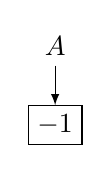
\begin{tikzpicture}[node distance=1cm,auto]
  \node (a) {$A$};
  \invb{b}{below of=a};

  \path[line] (a) -- (b);
\end{tikzpicture}
}

\newcommand{\pdiageig}{
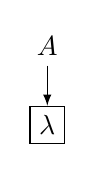
\begin{tikzpicture}[node distance=1cm,auto]
  \node (a) {$A$};
  \eigb{b}{below of=a};

  \path[line] (a) -- (b);
\end{tikzpicture}
}

\newcommand{\pdiageign}{
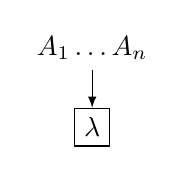
\begin{tikzpicture}[node distance=1cm,auto]
  \node (a) {$A_1 \ldots A_n$};
  \eigb{b}{below of=a};

  \path[line] (a) -- (b);
\end{tikzpicture}
}

\newcommand{\pdiagevec}{
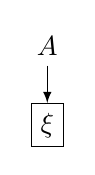
\begin{tikzpicture}[node distance=1cm,auto]
  \node (a) {$A$};
  \evecb{b}{below of=a};

  \path[line] (a) -- (b);
\end{tikzpicture}
}

\newcommand{\pdiagsvec}{
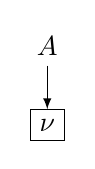
\begin{tikzpicture}[node distance=1cm,auto]
  \node (a) {$A$};
  \svecb{b}{below of=a};

  \path[line] (a) -- (b);
\end{tikzpicture}
}

\newcommand{\pdiagrot}{
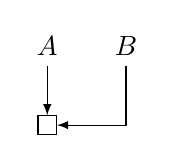
\begin{tikzpicture}[node distance=1cm,auto]
  \node (a) {$A$};
  \node[right of=a] (b) {$B$};
  \rotb{c}{below of=a};

  \path[line] (a) -- (c);
  \path[line] (b) |- (c);
\end{tikzpicture}
}

\newcommand{\pdiagwhite}{
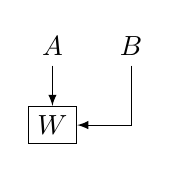
\begin{tikzpicture}[node distance=1cm,auto]
  \node (a) {$A$};
  \node[right of=a] (b) {$B$};
  \whiteb{c}{below of=a};

  \path[line] (a) -- (c);
  \path[line] (b) |- (c);
\end{tikzpicture}
}

